\subsection{Prototype \#2}
\label{sec:implementation:prototypes:prototype2}
\subsubsection{Purpose}
The purpose of the second prototype, 
was to test the indoor positioning of the user, 
using Estimote beacons, 
and determine if gesture recognition can be performed, 
using the hardware of a smartphone.

\subsubsection{Description}
The second prototype consisted of an iOS application, 
similar to the Android application described in \Cref{sec:implementation:prototypes:prototype1}, 
and a server that represented two controllable lamps.
The platform was changed from Android to iOS, 
because Estimote does not have a SDK for Android.

In this prototype the room was still represented as a grid, 
and the user was placed in the center of the grid, 
however the user was unable to change position.
This is because the first prototype showcased the idea of pointing at devices from different locations sufficiently, 
and the next step would be to use the actual location of a user using Estimote beacons.
As shown in \Cref{fig:prototype2-app-screenshots}, 
the user can see his direction as an angle between himself and north.
The angle is computed the same way as in Prototype 1 with \Cref{eq:angle}.

Devices are represented as orange dots, 
and if the user points towards one of them, 
two buttons will appear that allow the user to interact with the device, 
by either turning it \texttt{on} or \texttt{off}.
When the user turns a device on or off, 
it will be reflected on the server, 
where a corresponding box will have the color \texttt{green} when turned on, 
and \texttt{red} when turned off as shown in \Cref{fig:prototype2-server-screenshot}.
The server is running as a Heruko\footnote{\url{https://heroku.com/}} application, 
as a simple RESTful webservice written in Python. 
The server contains the information of the devices, 
such as ID, name, status and position.
The application gets this information by sending a GET request, 
to get a list of all the devices and their information. 
To change the status of a device (turn off or on), 
the application sends a POST request with the device's ID and the action. 
In this prototype, the only actions are \texttt{turnOn} and \texttt{turnOff}.

\subsubsection{Major Changes}
\begin{itemize}
    \item Introduction of a server for the application to interact with.
    \item Switched platform from Android to iOS.
\end{itemize}

\subsubsection{Results}

We were able to point at one or more devices,
and send an action to the devices, 
in order to flip between their two different states. 
Both the user's position and the devices were simulated.

The next step is to perform actual indoor positioning of the user.

\begin{figure}[!htb]%
    \centering
    \subfloat{
        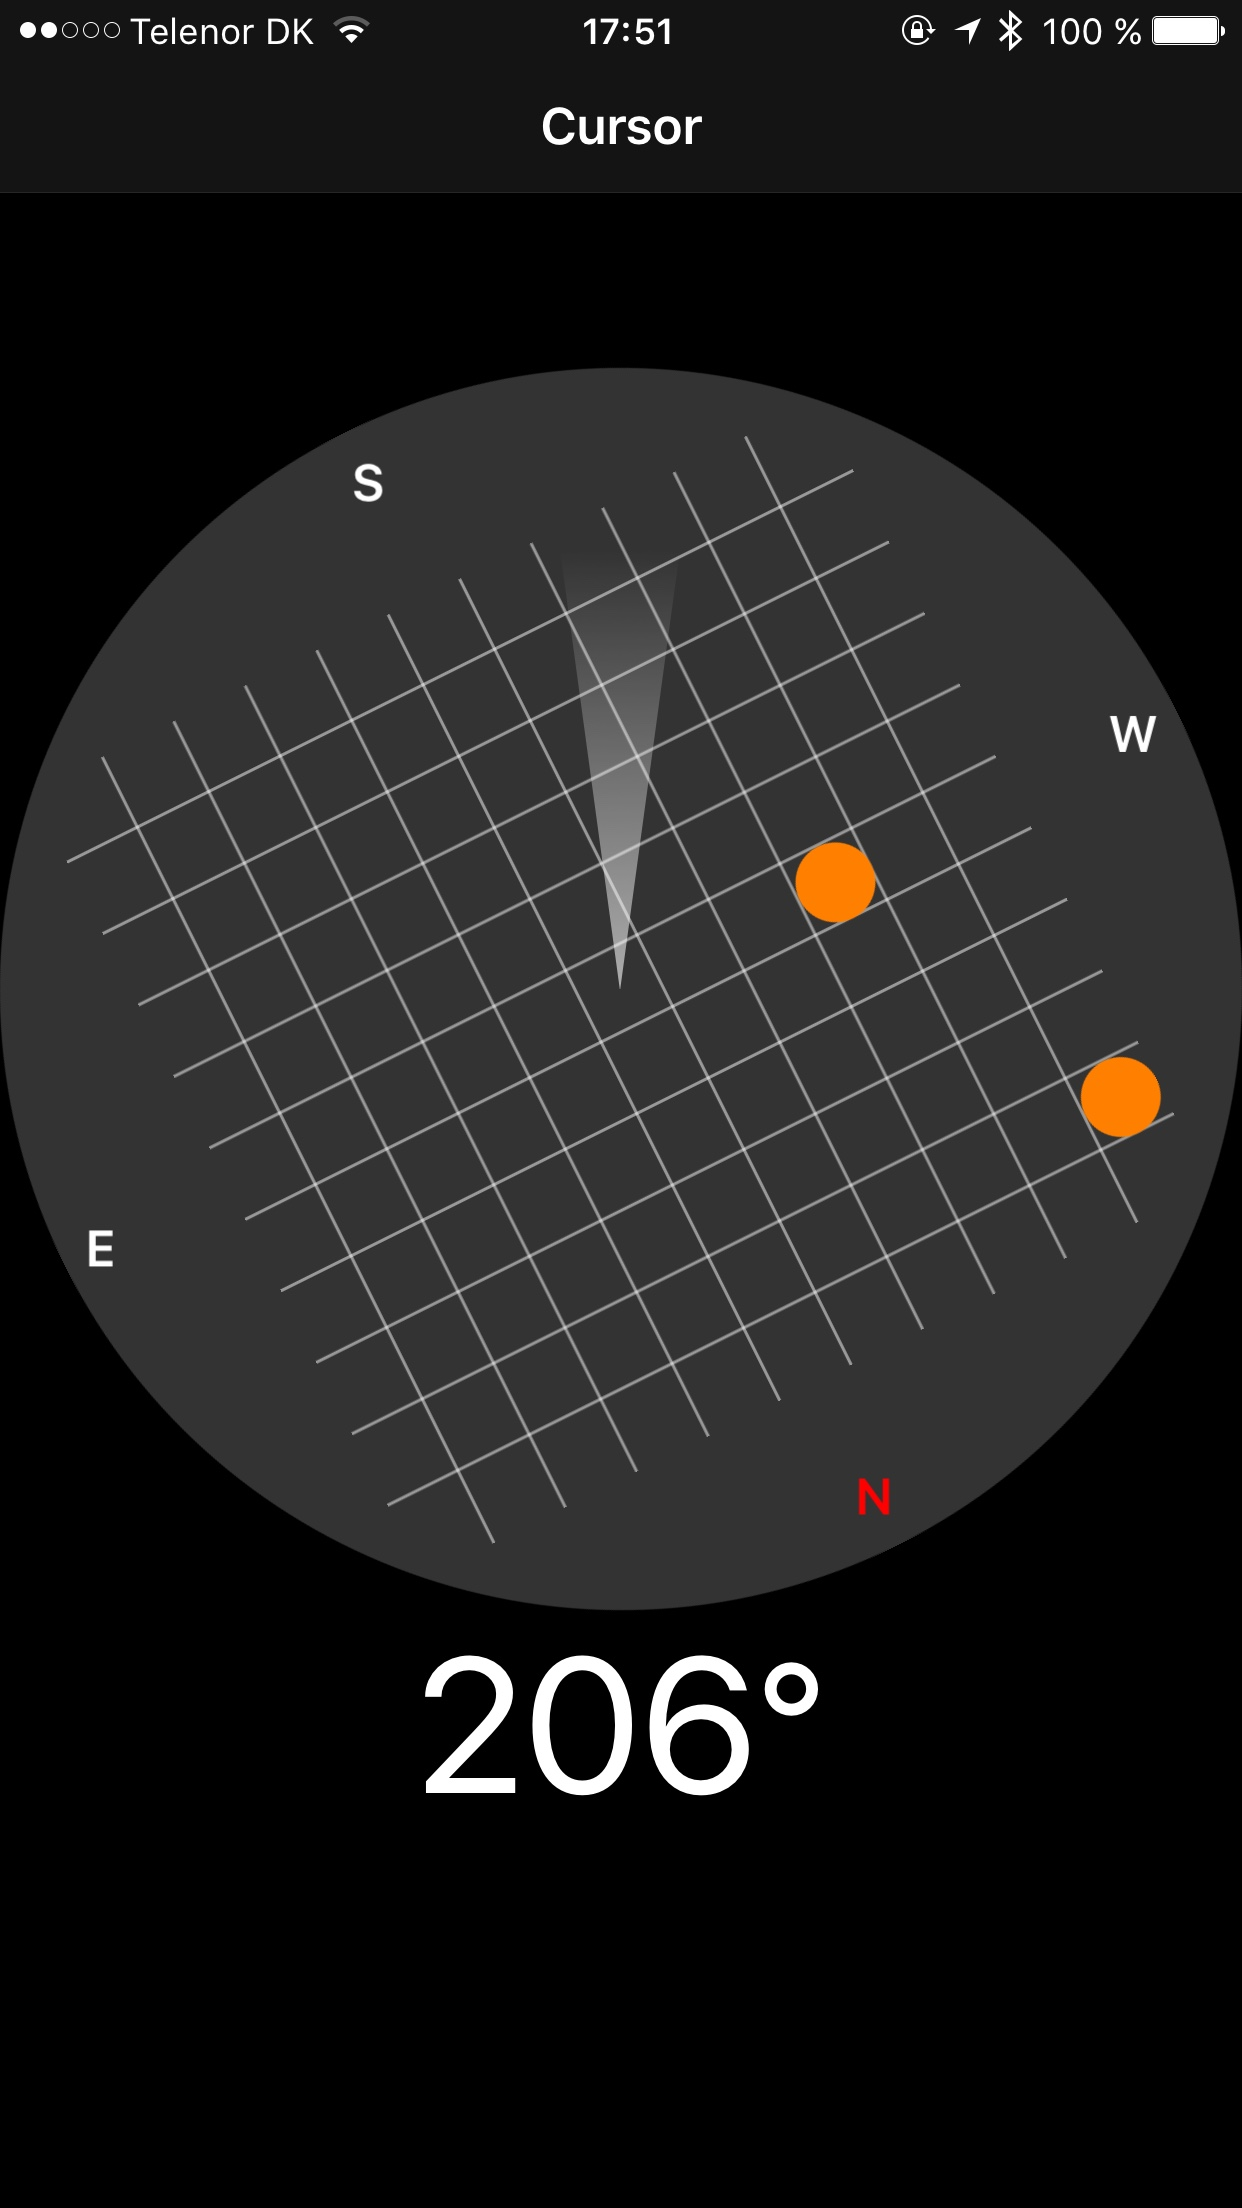
\includegraphics[width=0.3\textwidth]{images/Prototype2_iOS_1.png}
    }
    \subfloat{
        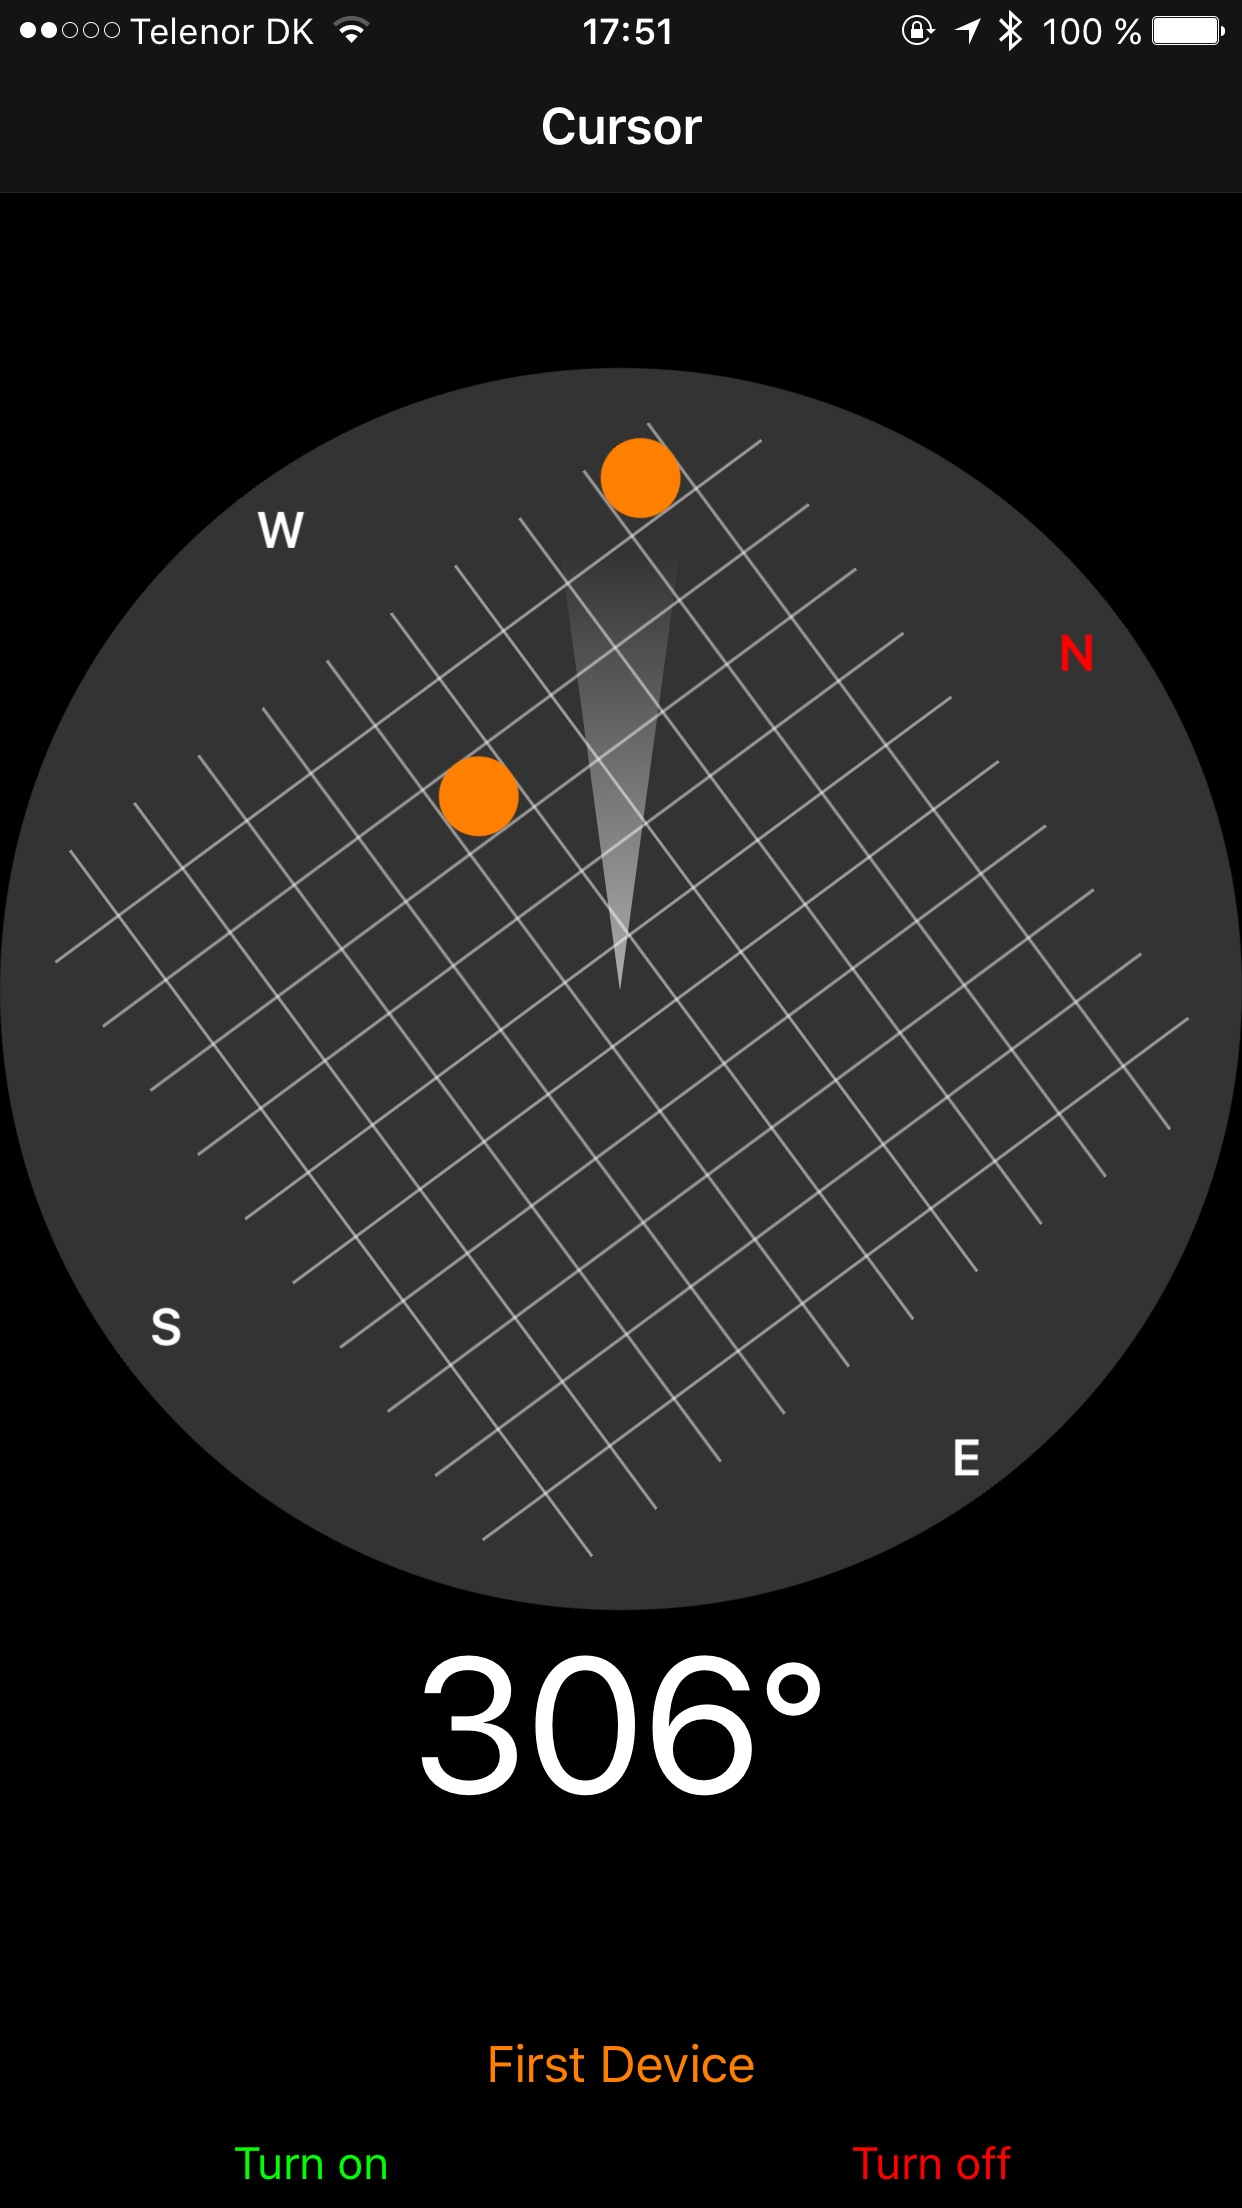
\includegraphics[width=0.3\textwidth]{images/Prototype2_iOS_2.png}
    }
    \caption{Screenshots of the second prototype application.}
    \label{fig:prototype2-app-screenshots}
\end{figure}

\begin{figure}[!htb]
    \centering
    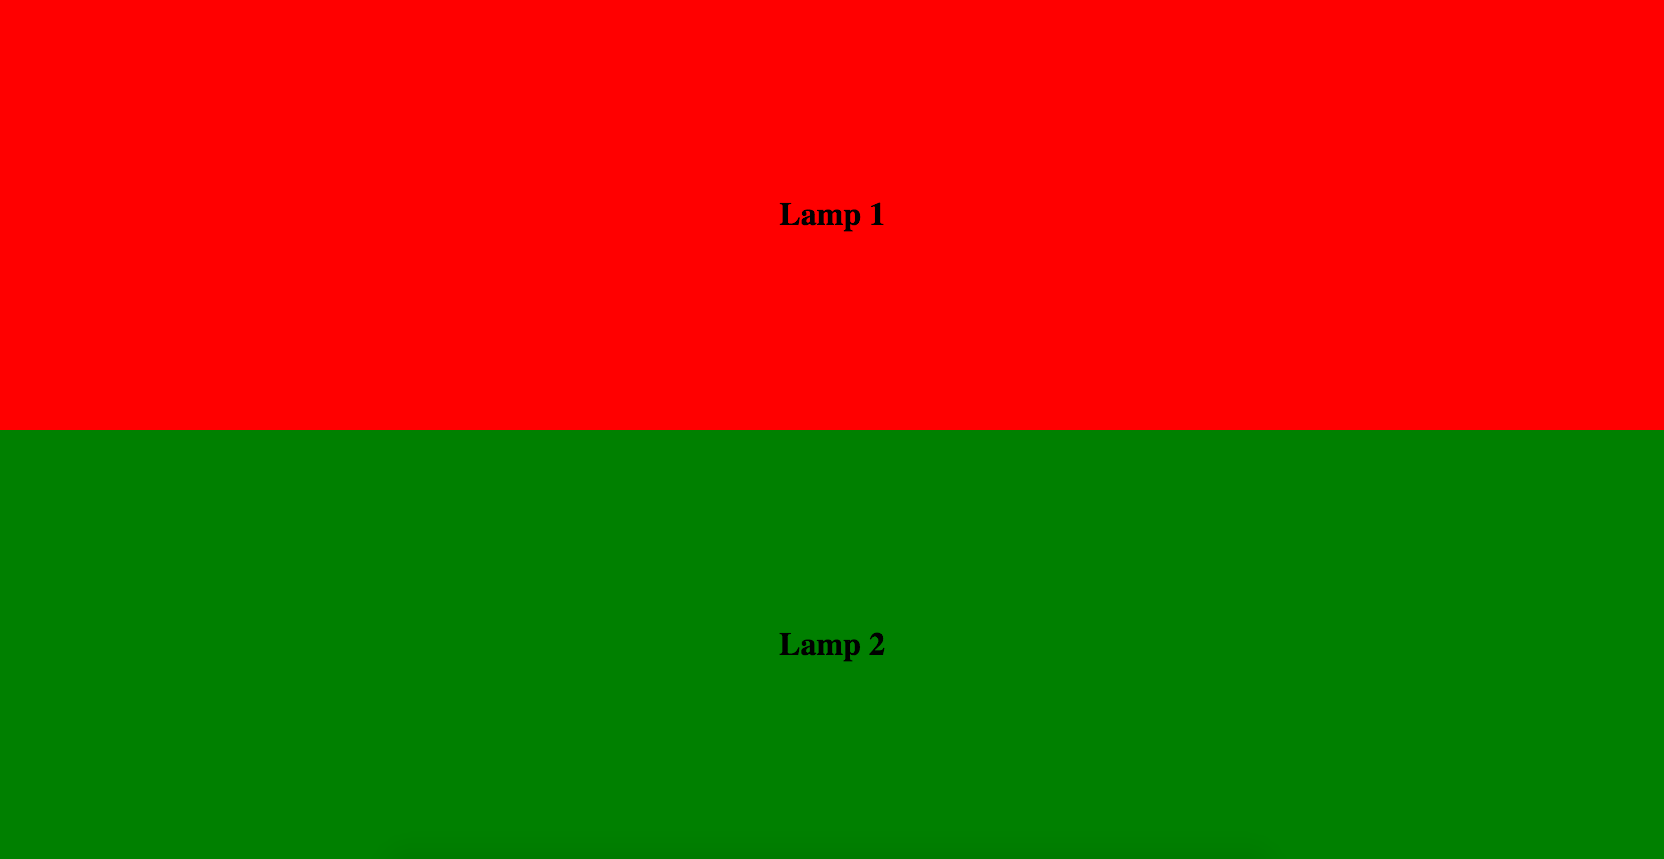
\includegraphics[width=0.8\textwidth]{images/Prototype2_Server.png}
    \caption{Screenshot of the server representing two lamps in the second prototype. Colors indicate their status. \texttt{Red} (top): Off and \texttt{Green} (bottom): On}
    \label{fig:prototype2-server-screenshot}
\end{figure}

%%% Local Variables:
%%% mode: latex
%%% TeX-master: "../../master"
%%% End:
